% !TEX encoding = UTF-8 Unicode
%!TEX root = thesis.tex
% !TEX spellcheck = en-US
%%=========================================
\chapter{Creating an Energy Efficient Platform}
\todo{more on embedded}
\label{chap:chapter2}

To create an energy efficient computer, there are two main parts to focus on, the Hardware and the Software.
Often they have to work together to create the best possible system.
This chapter will explain different energy saving techniques, by exploring both the Hardware and the Software view.

\section{Hardware}
\label{sec:hwenergy}
A very easy way of saving energy, is to let the computer run slower, executing fewer instructions.
As it is the act of executing an instruction that draws energy, running fewer instructions will lead to lower power use.
But as demonstrated by \fref{fig:energyusetime}, if the execution time of a program on a slower computer is long enough, the total energy use may be higher on a faster computer.

\begin{figure}[h]
\centering
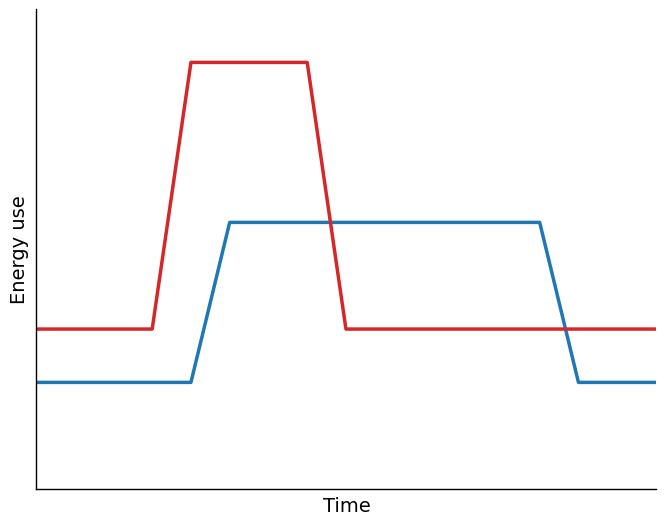
\includegraphics[scale=0.5]{fig/graphs/energyusetime.png}
\caption{Energy use of a fast processor (red) against a slow processor (blue) running the same program}
\label{fig:energyusetime}
\end{figure}

To exploit this behavior, dynamic scaling of the clock, as well as the input voltage, can be used.
By letting the operating system gather data from performance- and energy-critical events, the operating system can manage the demands from each application. \citep{Weissel2002}
Later research has found that the gain from dynamic frequency scaling has diminished, for instance sleep states in processors has become better.\citep{lesuer2010}

Sleep state is another name for low power states, where less of the computers resources are available.
While waiting for input, for instance, the CPU does not need to be running with nothing to do.
Doing so is called busy-wait, and consumes a lot of energy, because much time is spent in a loop where the only thing done is checking if input has happened yet.
It is the computer equivalent to children on a road trip constantly asking ``are we there yet?''
Introducing \emph{interrupts} is a better concept, where the application tells the operating system that it is waiting for an interrupt.
The OS can then either schedule other programs to run, or turn off resources that are not needed to wake up again, i.e. enter a sleep state.
When the interrupt is fired, the OS returns control to the application, through an interrupt handler which gets the input, and resumes the running of the program.
In input heavy programs, where the time spent waiting for input dominates the calculation time, a lot of energy can be saved by using sleep sates.

\begin{figure}[h!]
\centering
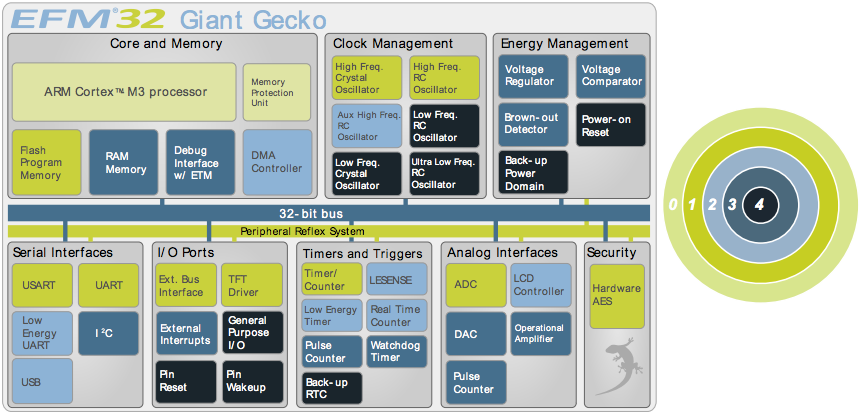
\includegraphics[scale=0.4]{fig/pics/EFM32EM.png}
\caption{The energy modes of the Silicon Labs EFM32 Giant Gecko}
\label{fig:efm32em}
\end{figure}

\defcitealias{silabsefm32ref}{EFM32 Giant Gecko Reference Manual, 2014}
\defcitealias{efm32gg990ds}{EFM32 Giant Gecko 990 Datasheet, 2014}
For example, the Silicon Labs EFM32 Giant Gecko has five energy modes with different hardware capabilities available in the different modes, as shown in \fref{fig:efm32em}.
EM0 is the normal running mode, where the CPU is available.
In figure \ref{fig:efm32em} it is shown in light green.\citepalias{silabsefm32ref}
The use of these energy modes does have some drawbacks, namely that it takes time to wake up from the deeper sleep modes.
On the EFM32GG990 device, it takes 163\si{\micro\second} to wake up from the deepest sleep mode, which might cause problems in timing sensitive systems.
In addition, it also consumes more energy to wake up from a sleep state.\citepalias{efm32gg990ds}

Because of the failure of Dennard Scaling (stating that faster transistors and more of them on a chip leads to progress) in recent years, the term \emph{dark silicon} has been introduced. 
When more and more transistors are running on a single chip, the heat of the device becomes to great too sustain, and some parts of the chip must be turned off, or kept dark.
This is a disadvantage when the goal is to use as much of the chip at one time as possible, but research is being done into leveraging this property when designing the system, i.e. purposely turn off some parts of the chip that can be beneficial. \citep{Taylor:2012:DSU:2228360.2228567}

\citet{kumar2003} created an architecture for multiple heterogeneous cores, using existing cores with a similar instruction set.
By using an informed strategy for choosing the core to run the program on, and having the ability to switch core dynamically while running, they achieve an increase in energy efficiency.
Similarly, the SHMAC (The Single-ISA Heterogeneous MAny-core Computer)\footnote{http://www.ntnu.edu/ime/eecs/shmac} project tries to create a computer with multiple different cores.
However, some cores are more capable of specific tasks than others, using accelerators, out-of-order processors or vector processors.
The computer can then allocate a specific core for a task, and turn off the cores that are not used. 
This can save energy in the same way as \citet{kumar2003}, while at the same time achieve a performance boost by using specialized hardware. \citep{jahreshmac}

\section{Software}
Running optimized code on the platform might lead to lower power consumption, as shown by \citet{kavvadias04} and \citet{valluri01}. 
A compiler can perform many different optimizations, some common are listed below. \citep[chap. 9]{dragon}

\begin{description}
\item[Global common subexpression] \hfill \\
    Find some subexpression in the code that is calculated multiple places, and instead only calculate it once, putting the result of the calculation into the places that redundantly calculated the expression.
\item[Constant folding] \hfill \\
    Deducing that some variable or calculation is constant, and replacing it with the constant.
\item[Dead code elimination] \hfill \\
    Finding that some part of the code is unreachable at run-time, and instead of having to add this parts to the compiled code, it can be eliminated.
\item[Function inlining] \hfill \\
    Copying the code in a function to the place it was called, to remove the added work of calling a function.
\item[Loop unrolling] \hfill \\
    Reduce the number of iterations in a loop by doing more work in each iteration, for example do the calculations for originally three iterations in one.
\item[Code-motion] \hfill \\
    Find loop-invariant code, i.e. calculations that does not need to be calculated for each iteration in the loop, and move it oustide the loop body.
\item[Reduction in strength] \hfill \\
    Swap an expensive instruction for a cheaper one.
\end{description}

The strength of these optimization becomes apparent when they are applied together, and also multiple times.
For instance, after a function inlining, some expression in the code that was former the function can be a constant, which could lead to some code in the function being dead.
As shown by \citeauthor{delima13}, the order of the techniques can impact the results of the optimization.

An interpreter executes the code as it runs, and it cannot get the insight a compiler does to perform optimizations.
If the interpreter were to perform the same techniques, it would have to do two passes of the code, and the whole purpose of the interpreter would vanish.
But there is a middle ground, called \emph{just-in-time compilation}, or JIT compilation for short.

A JIT compiler runs as the program is executing, just like an interpreter.
But it does not necessarily only translate one expression at a time, it can compile larger blocks, allowing for optimizations on these parts before they are executed.\citep{Aycock:2003:BHJ:857076.857077}


Another way of making the software save energy, is to not execute code at all.
With the rise of Internet connected devices, it has become feasible to load off the computation heavy operations to some other computer.
A common example of this is making a server create queries and retrieve data from a database, which might be computation intensive.
A newer example is in gaming, where a handheld device gets rendered 3D data from a dedicated gaming computer as a video stream, and sends input signals back.
The PlayStation Vita\footnote{https://www.playstation.com/en-us/explore/psvita/}, made by Sony, is a small gaming device, that is able to play any PlayStation 4 game through network connection, despite not being powerful enough to render the games.